\chapter{Parallel computation of the exposure map}
\label{appendix:exposure}

A long calculation time from the exposure calculation came from 
two matrix transformations to accumulate the LAT exposure time 
when it sees the Earth. Since the FT2 or spacecraft log file is
recorded in the position and all metadata.

For each step time, 
the transformation matrix will be calculated from a the 
information of spacecraft orientation.
After that, each grid-like nadir angle 
that represented in equatorial coordinate (Equation \ref{eq:def_r0})
was transformed into the plane of detector (Equation \ref{eq:def_r0_to_rp}).
Hence, we can inspect the incidental from a given nadir angle
for summing the LAT exposure time and multiples with 
the effective area in the visible region.

There is one thing that could be used to approximate the 
complexity of the code which is the resolution of the exposure map.
Assuming that there are M cells in $\theta_\text{NADIR}$ axis
and N cells in $\phi_\text{NADIR}$ axis. It will cost 
$\mathcal{O}(MN)$ multiply by the complexity of two 
transformation matrices to compute a single exposure map.
Last but not least, this complexity will be multiplied by 50 times 
since we have 50 bins that have their own specific mean energy 
which affects the effective area.


The first version of Python code takes 1434.76 seconds to finish 
one week of FT2 data.
% There are 531 weeks to calculate, then 
% it will take around 9 days to finish this task.
In addition, the matrix transformation is already used Numpy 
for all matrix operations which means that the plain Python code 
likely to takes longer than this speed. In the meantime, using 
serial code with C++ takes around 11.85 seconds to finish 
the workload of a single week. Meaning that the calculation time 
is $\sim$120 times faster from the compiling language.

The parallel code is implemented in the C++ programming language 
with Message Passing Interface (MPI). We use Master-Slave techniques
for fully utilizing the CPU resources where the master process 
is monitoring and sending the task to all workers. Consequently,
there is only one master process and allows the program scale 
horizontally by adjusting the number of slave processes. 

\begin{figure}[h]
    \centering
    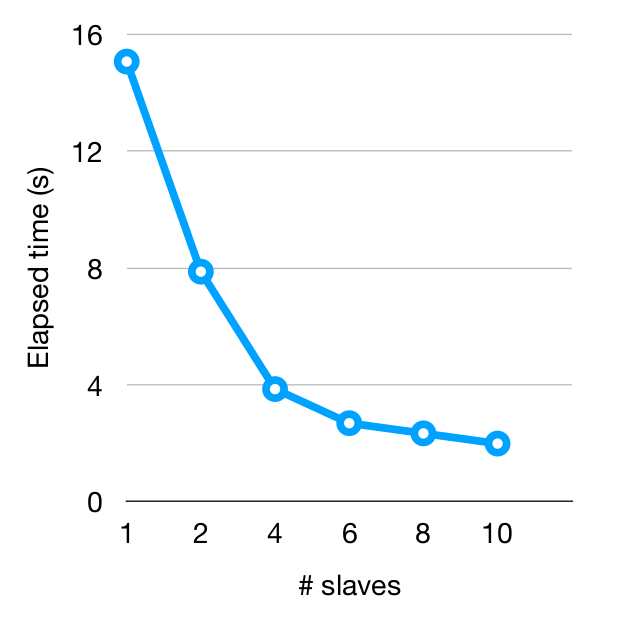
\includegraphics[width=0.6\textwidth]{appendix/exposure/ms_perf.png}
    \caption{
        Benchmarking of the serial and parallel code
        in the low level language.
    }
    \label{fig:parallel_benchmark}
\end{figure}

The hardware that was used to benchmark compose of 6 cores and 
12 threads. Figure \ref{fig:parallel_benchmark} shows the 
scalability of the code in the exponential trends of 
the elapsed time and the number of slave processes.
The underlying reason why it became a plateau curve on the 
edge came from the maximum available running threads on this hardware
is only twelve which means that the more number of worker that 
excess this limit does not reduce the computation time.
However, the total CPU cores on the cluster in space
physics laboratory are around 200 thread executors.
The performance from running the parallel code in the cluster 
takes only a dozen hours to finish.


